%%%%%%%%%%%%%%%%%%%% author.tex %%%%%%%%%%%%%%%%%%%%%%%%%%%%%%%%%%%
%
% sample root file for your "contribution" to a contributed volume
%
% Use this file as a template for your own input.
%
%%%%%%%%%%%%%%%% Springer %%%%%%%%%%%%%%%%%%%%%%%%%%%%%%%%%%


% RECOMMENDED %%%%%%%%%%%%%%%%%%%%%%%%%%%%%%%%%%%%%%%%%%%%%%%%%%%
\documentclass[graybox]{svmult}

% choose options for [] as required from the list
% in the Reference Guide

\usepackage{mathptmx}       % selects Times Roman as basic font
\usepackage{helvet}         % selects Helvetica as sans-serif font
\usepackage{courier}        % selects Courier as typewriter font
\usepackage{type1cm}        % activate if the above 3 fonts are
                            % not available on your system
%
\usepackage{makeidx}         % allows index generation
\usepackage{graphicx}        % standard LaTeX graphics tool
                             % when including figure files
\usepackage{multicol}        % used for the two-column index
\usepackage[bottom]{footmisc}% places footnotes at page bottom

\usepackage{natbib}
\usepackage{aas_macros}

% see the list of further useful packages
% in the Reference Guide

% Added:

\usepackage{ amssymb }


\makeindex             % used for the subject index
                       % please use the style svind.ist with
                       % your makeindex program

%%%%%%%%%%%%%%%%%%%%%%%%%%%%%%%%%%%%%%%%%%%%%%%%%%%%%%%%%%%%%%%%%%%%%%%%%%%%%%%%%%%%%%%%%

\begin{document}

\title*{Long baseline imaging with LOFAR}
% Use \titlerunning{Short Title} for an abbreviated version of
% your contribution title if the original one is too long
\author{Javier Mold\'{o}n and Eskil Varenius}
% Use \authorrunning{Short Title} for an abbreviated version of
\authorrunning{J. Mold\'{o}n and E. Varenius}
% your contribution title if the original one is too long
\institute{Javier Mold\'{o}n \at ASTRON, Postbus 2, 7990 AA Dwingeloo, The Netherlands, \email{moldon@astron.nl}
\and Eskil Varenius \at Onsala Space Observatory, Dept. of Earth and Space Sciences, Chalmers University of Technology, SE-43992 Onsala, Sweden  \email{varenius@chalmers.se}
}
%\and Name of Second Author \at Name, Address of Institute \email{name@email.address}}
%
% Use the package "url.sty" to avoid
% problems with special characters
% used in your e-mail or web address
%
\maketitle

\abstract*{In this chapter we focus on the calibration of International LOFAR,
which includes the long baselines provided by international stations, to produce
high-resolution radio images. The Very Long Baseline Interferometry (VLBI)
techniques are explained, as well as the different steps required to properly
calibrate a long-baseline observation at low frequencies.}

%\abstract{In this chapter we focus on the calibration of International LOFAR,
%which includes the long baselines provided by international stations, to produce
%high-resolution radio images. The Very Long Baseline Interferometry (VLBI)
%techniques are explained, as well as the different steps required to properly
%calibrate a long-baseline observation at low frequencies.}

% Learning Specifics
% In this chapter we focus on the calibration of International LOFAR, which includes
% the long baselines provided by international stations, to produce high-resolution
% radio images. The Very Long Baseline Interferometry (VLBI) techniques are ex-
% plained, as well as the different steps required to properly calibrate a long-baseline
% observation at low frequencies.
% Learning Objectives
% -  To understand the key differences between short- and long-baseline interferome-
% try.
% -  To understand the scales for LOFAR VLBI: resolution and field of view.
% -  To understand the variables relevant for long baseline interferometry: phase, de-
% lay, delay rate.
% -  To understand the impact of baseline separation, ionosphere, and source structure
% on the phase behavior.
% -  To understand how the phase calibration is conducted in VLBI.
% -  To know what calibrators are needed in a typical long baseline observation.
% -  To understand the differences between cm-VLBI and m-VLBI. To understand
% the dispersive delay produced by the ionosphere.
% -  To know how to form a sensitive tied station from the LOFAR core stations.
% -  To understand why circular polarization is useful and how to convert the data.
% -  To know how to combine sub-bands in a measurement set to form a FITS file.
% -  To know how to manage FITS files, convert them, and manipulate them in AIPS.
% -  To know how to conduct a VLBI phase calibration in AIPS.
% -  To know how to inspect phase solutions and to understand their meaning.
% -  To know possible ways to obtain the amplitude calibration for international sta-
% tions.
% -  To know how to produce high-resolution radio images.

\section{Introduction}
\label{sec:introduction}

In this chapter we focus on the calibration of International LOFAR, which
includes the long baselines provided by international stations, to produce
high-resolution radio images. The Very Long Baseline Interferometry (VLBI)
techniques are explained, as well as the different steps required to properly
calibrate a long-baseline observation at low frequencies. Some of the
discussions will be focused on the LOFAR HBA, since currently the LBA
calibration process is still not well understood and optimized.

% JM: I have to think about a few lines with science motivation

\section{Long baselines with International LOFAR}

Observations with the LOFAR international stations are mainly different from
the Dutch array observations in that station separations above 200~km provide
different scales that require different approaches. The main differences in the
array itself are that the density of stations is scarce, and provides a less
dense uv-coverage, that the instrument has a much reduced field of view (FoV),
and that the atmospheric conditions above each station are highly uncorrelated,
making the phase calibration much more delicate. The majority of the LOFAR
stations, namely the core and remote stations, are distributed over an area
roughly 180 km in diameter predominantly in the northeastern Dutch province of
Drenthe. Currently, the array also includes 8 international LOFAR stations
across Europe that provide maximum baselines up to 1292~km. One additional
station is planned to be completed in Hamburg (Germany) in 2014, and three
stations in Poland will commence construction in 2014, extending the maximum
baseline to $\sim$2000~km. Fig.~\ref{fig:stations} shows the distribution of
current and planned stations of International LOFAR.

%\footnote{An up-to-date map of all LOFAR stations can be found at \url{http://www.astron.nl/~heald/lofarStatusMap.html}.}.  

\begin{figure}[t]
%\sidecaption[t]
\begin{center}
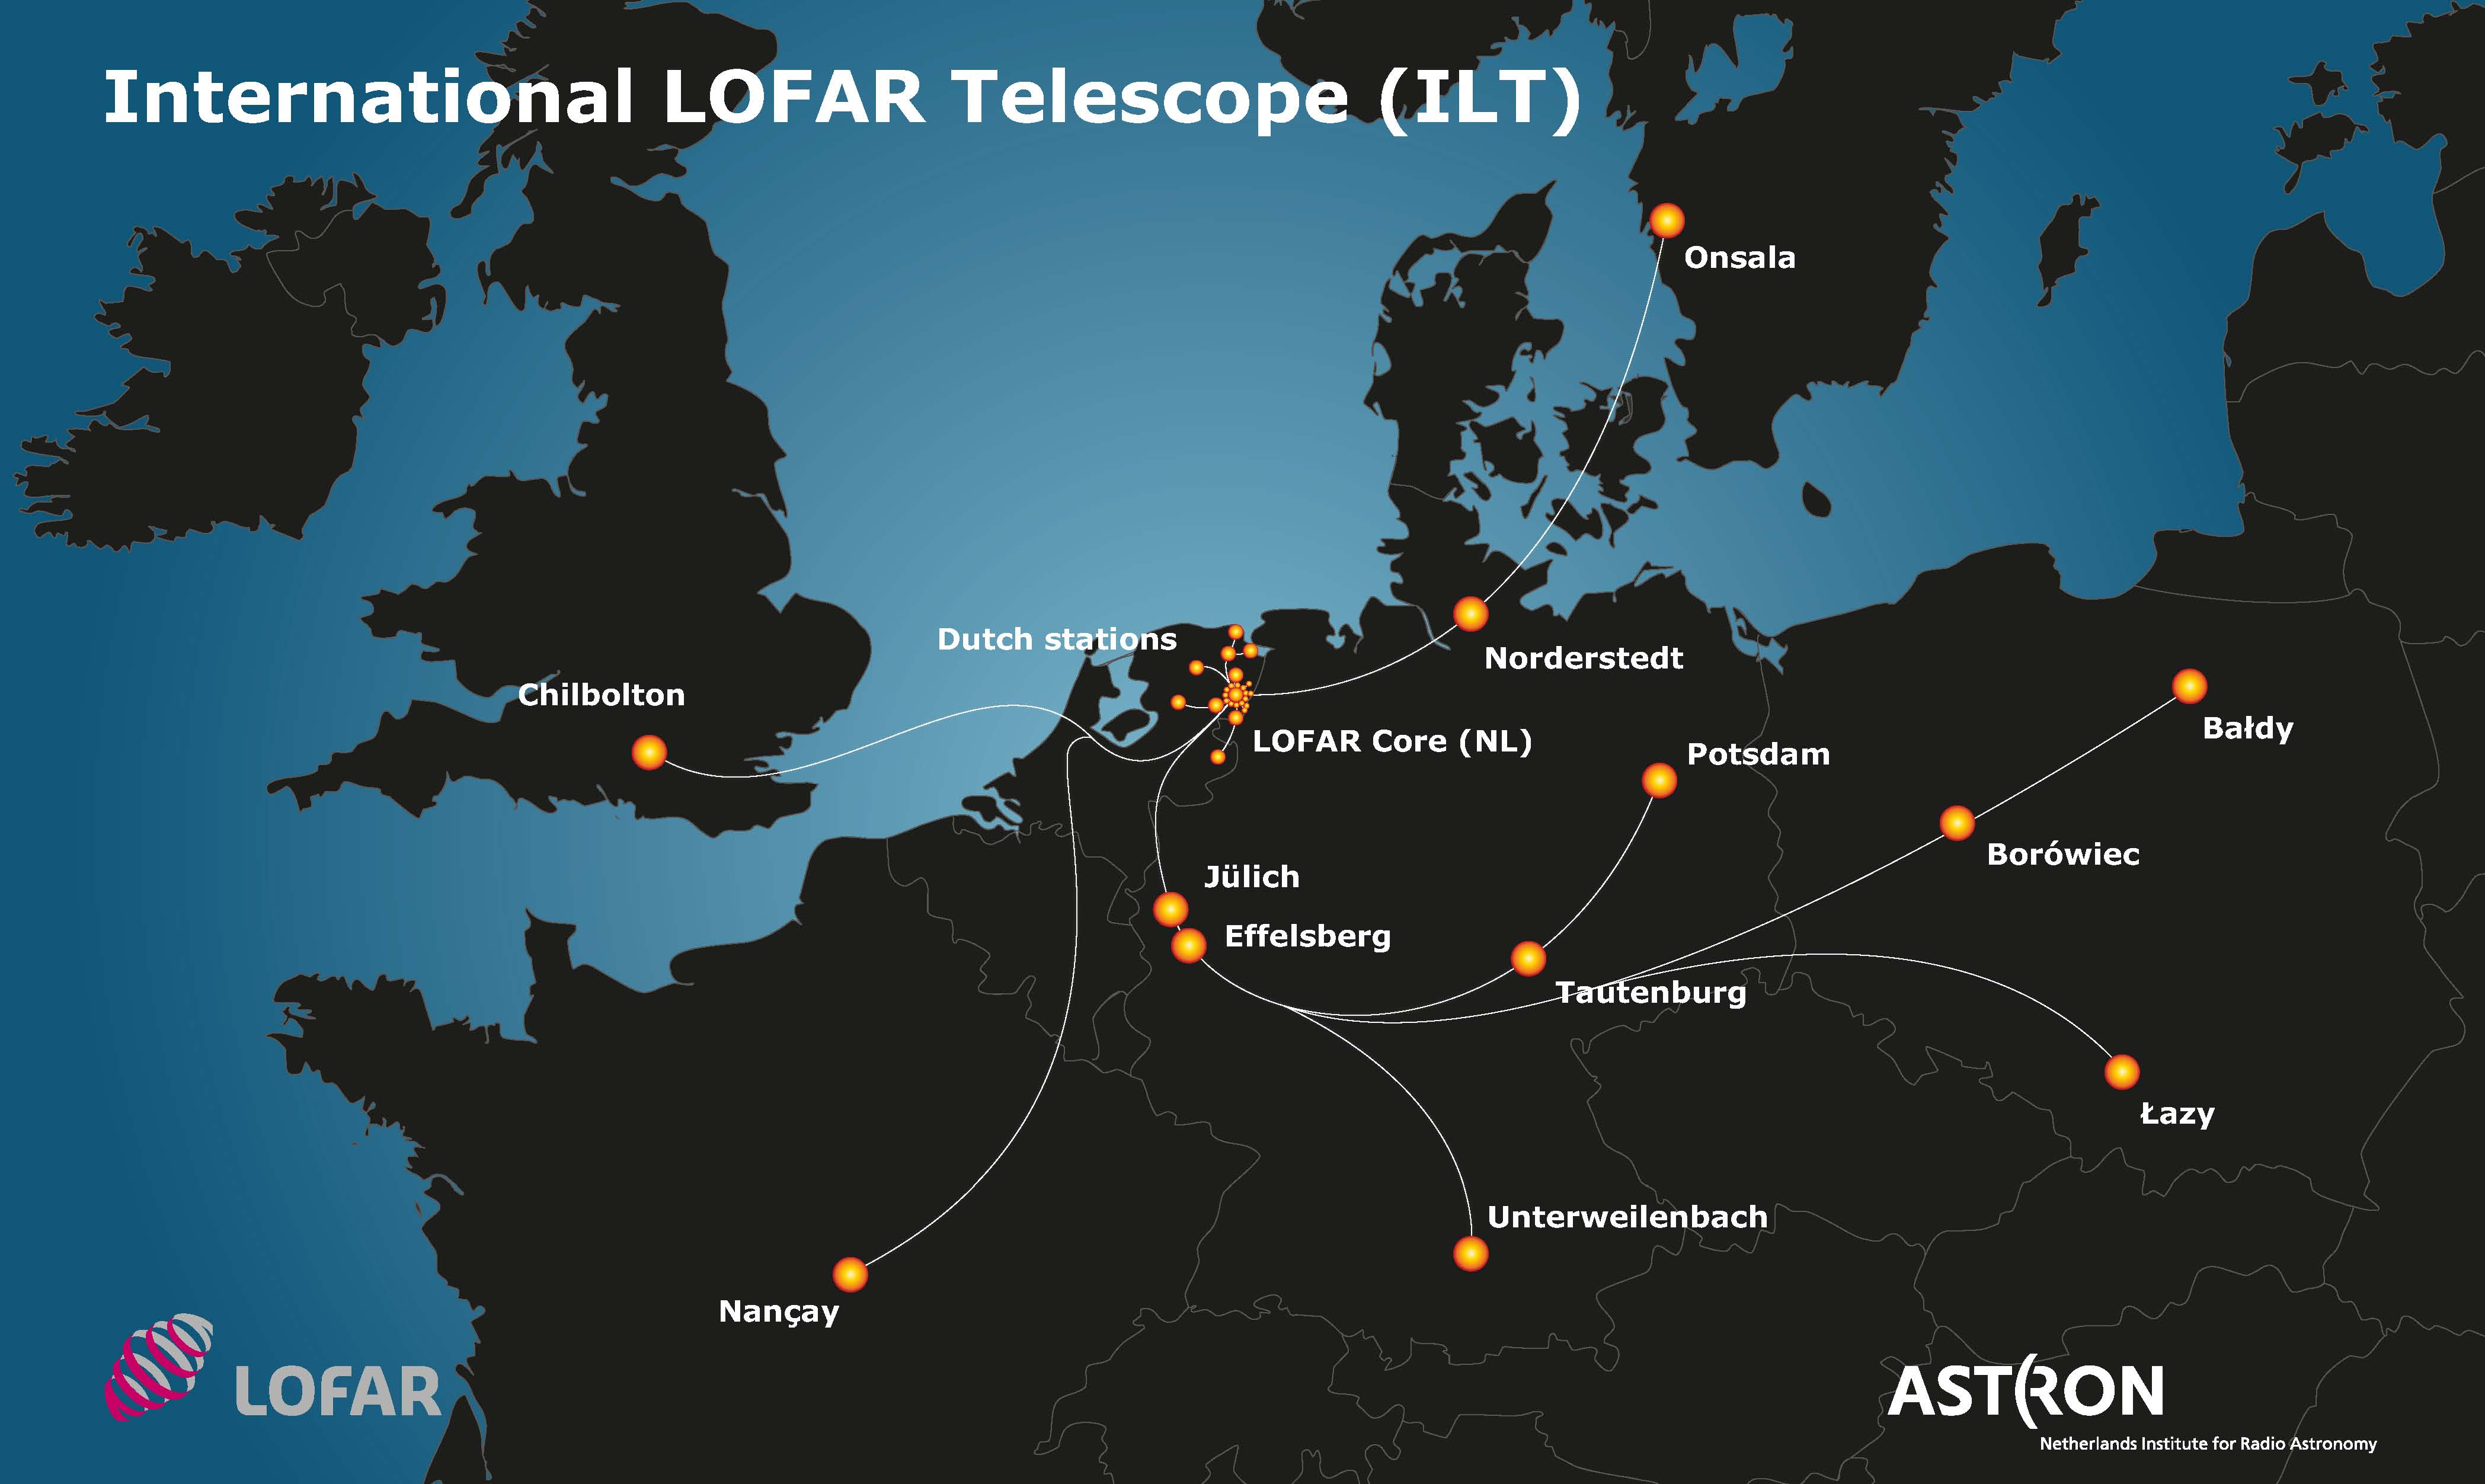
\includegraphics[width=8cm]{figures/LOFAR_stations_map.jpg}
\caption{LOFAR is composed by 24 core stations and 13 remote stations in the
Netherlands, and 8 (+4 planned) international stations.}
\label{fig:stations}
\end{center}
\end{figure}

\subsection{uv-coverage}\label{sec:uvcoverage}

The maximum baseline of an interferometer determines the spatial resolution of
the instrument. The core stations provide maximum baselines of 2.7~km, the
remote stations up to 120~km, and the international stations of 1300~km.
Table~\ref{tab:baselines} shows the distances between each pair of international
stations, and CS001 as a reference of the location of the center of the array.
However, the density of visibilities in the $uv$ space determines the fidelity
of the image. The LOFAR core provides a very dense $uv$ sampling, but at the
longest $uv$ distances it is much more scarce. A typical LOFAR $uv$ coverage is
shown in Fig.~\ref{fig:uvcoverage}. We can see that the sampling covers 3 orders
of magnitude in $uv$ distance.


\begin{table}[h]
\centering
\begin{tabular}{cccccccccc}
\hline
\hline
      & CS001& DE601& DE602& DE603& DE604& DE605& FR606& SE607& UK608\\
\hline
 CS001&     0&   266&   581&   396&   419&   226&   700&   594&   602 \\
 DE601&   266&     0&   390&   344&   476&    53&   490&   833&   590 \\
 DE602&   581&   390&     0&   277&   455&   440&   690&   990&   959 \\
 DE603&   396&   344&   277&     0&   186&   372&   800&   714&   920 \\
 DE604&   419&   476&   455&   186&     0&   487&   957&   556&  1005 \\
 DE605&   226&    53&   440&   372&   487&     0&   498&   807&   552 \\
 FR606&   700&   490&   690&   800&   957&   498&     0&  1292&   495 \\
 SE607&   594&   833&   990&   714&   556&   807&  1292&     0&  1110 \\
 UK608&   602&   590&   959&   920&  1005&   552&   495&  1110&     0 \\
\hline
\end{tabular}
\caption{Separation in km between the main core and the currently available
international stations.
\label{tab:baselines}}
\end{table}

% JM: If enough space, this plot can have 2x2 panels for better visibility.
% JM: it is possible to use different colors for CSCS, RSRS, etc. For visual
% simplicity, I would use at most one additional color for the CSCS baselines.
\begin{figure}[t]
\begin{center}
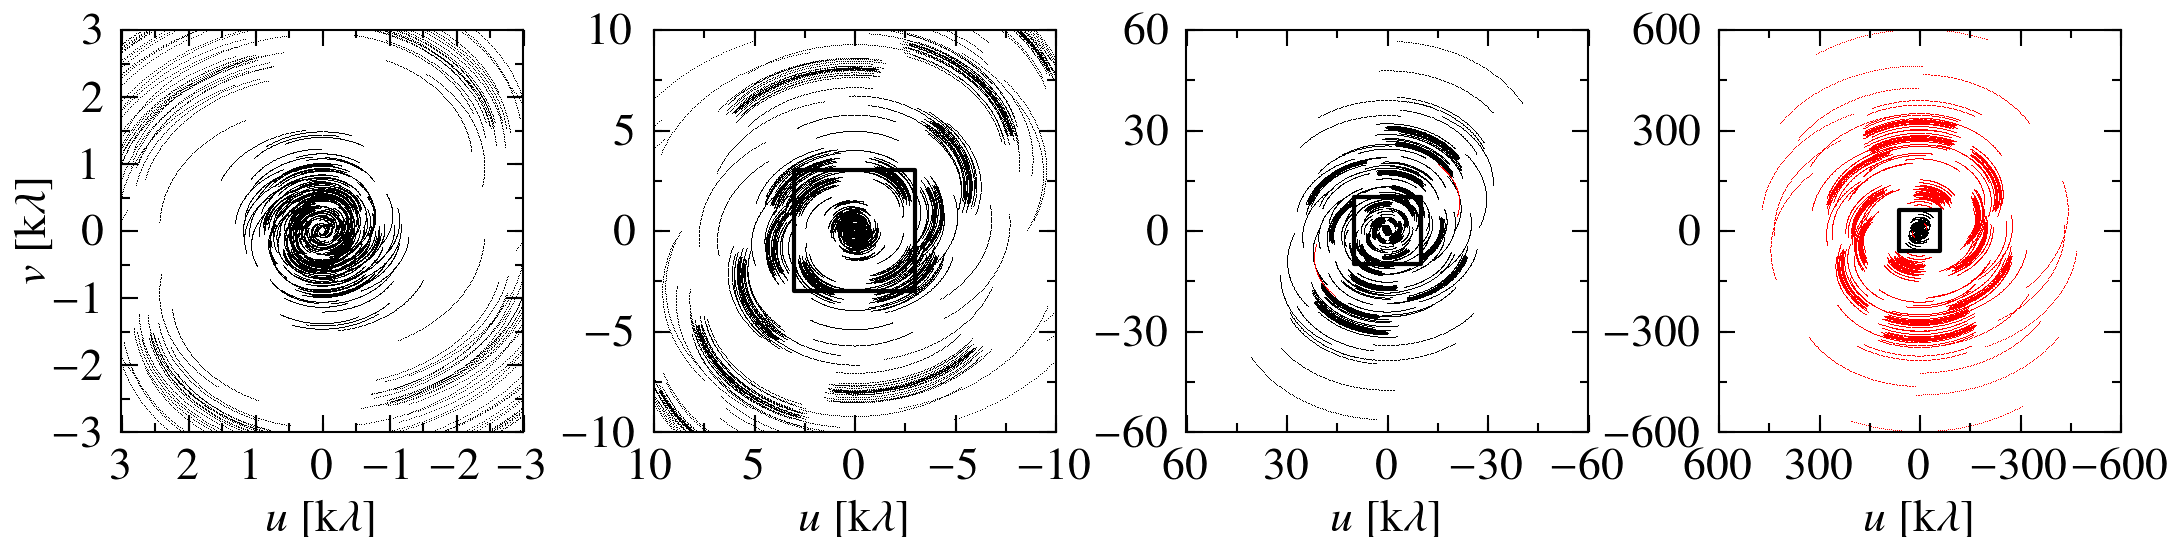
\includegraphics[width=\textwidth]{figures/uv_cov.png}
\caption{$uv$ coverage for a typical 4-hr observation of a source at declination
$+48^{\circ}$ with a single subband centred at 140~MHz. Only one visibility every 160 seconds is shown. The rectangles in the last three panels show the area covered by the previous panel. Visibilities corresponding to baselines with international
stations are plotted in red.}
\label{fig:uvcoverage}
\end{center}
\end{figure}

%
%\begin{table}
%\caption{Current international LOFAR stations}             % title of Table
%\label{tab:ilofarstations}      % is used to refer this table in the text
%\centering                          % used for centering table
%\begin{tabular}{l c c} 
%\hline\hline
%Station & Distance to  &  Corresponding resolution  \\
%        & LOFAR core (km) &  at 140 MHz ($^{\prime\prime}$) \\
%\hline
%DE605  & 226  &  2.4  \\
%DE601  & 266  &  2.0  \\
%DE603  & 396  &  1.4  \\
%DE604  & 419  &  1.3  \\
%DE602  & 581  &  0.9  \\
%SE607  & 594  &  0.9  \\
%UK608  & 602  &  0.9  \\
%FR606  & 700  &  0.8  \\
%\hline                                   %inserts single line
%\end{tabular}
%\end{table}


\subsection{International LOFAR field of view (FoV)}\label{sec:fov}

The area possible to image in a single LOFAR observation (NL or international)
is limited by several factors such as the station beam, geometrical/projection
effects, such as W-projection artefacts, variations in the atmosphere within
the image, and averaging of visibility data, also referred to as time and
frequency \emph{smearing}. Here we will focus on describing the latter.

Since correlators output a discrete set of visibilities (i.e. samples in time
and frequency), averaging is to some extent always done on interferometric
data. We may also average the data further after correlation to reduce the
computational resources needed for calibration and imaging. Any averaging must
however be done with care.  Averaging a range of samples in time and frequency
together corresponds to averaging over a small parallelogram in Fourier space.
This means some information is lost, and one has to take care to not lose
information that could affect the scientific results. For LOFAR, the standard
\emph{raw} data are delivered from the correlator with resolution 1 second in
time, and 64/channels per subband.  Each subband (using the standard 200\,MHz
clock) is 195\,kHz wide, meaning that the default minimum averaging bandwidth is
3~kHz. This will limit the dynamic range at some distance from the observed
phase center, similar to the station beam effects described above.  A detailed
description of the averaging losses is beyond the scope of this chapter, we
merely quote the often used results by \cite{taylor99} 
chapter 18, who derived two expressions to estimate the average amplitude loss
due to averaging in frequency and time, at some distance from the phase center.
For frequency smearing, we can use their expression 18-24 assuming a square
bandpass and circular Gaussian tapering, where the reduction in amplitude can
be estimated as

\begin{equation}
\frac{I}{I_0} = \frac{\sqrt{\pi}}{2\sqrt{\ln{2}}}\frac{\theta \nu_c}{r \Delta
\nu}\mathrm{erf}\left(\sqrt{\ln{2}}\frac{r \Delta\nu}{\theta \nu_c}\right)
\label{eqn:freqloss}
\end{equation}

where $\theta$ is the synthesized beam size (FWHM), $\nu_c$ is the central
frequency of the observation, $r$ is the distance from the phase center, and
$\Delta \nu$ is the bandwidth. Note that the units of $\theta$ and $r$ cancel
if they are given in the same unit. Note also that this expression is in fact
independent of central frequency $\nu_c$ since the synthesised beam also scales
with $\nu_c$, only the bandwidth is important.

For time smearing, we may use their formula 18-43, assuming a 12 hour average
over a circular UV-coverage with Gaussian tapering:

\begin{equation}
\frac{I}{I_0} = 1-1.22\times 10^{-9}\left(\frac{r}{\theta}\right)^2\tau_a^2
\label{eqn:timeloss}
\end{equation}
where $\tau_a$ is the averaging time in seconds.
%JM: We use tau for the delay. Maybe we should use delta(t)

What loss to define as acceptable of course depends on your science, in
particular the brightness of your target, but as a general guide one may
tolerate 5\% loss in amplitude due to averaging. Using the standard LOFAR raw
data values, we have calculated the corresponding circle (diameter, to compare
with station FWHM) for different observing frequencies, see Table
\ref{tab:res}. We note that, except for the lowest LBA frequencies, we are
limited by time averaging, where the 5\% loss diameter is smaller than the
station beam. Note that this limitation is not present for shorter baselines,
and usually not a cause for worry in NL-LOFAR observations. But, with the
longest baselines, the main restriction may (if you need excellent sensitivity)
be the averaging by the raw data. 
% ** NOTE **
% JM: It could be interesting to include some more columns, since there is
% space. For example 20% loss, or add 4s averaging and 4ch/subband. Check
% numbers and decide if including them or not.
% JM: another possibility is to do a plot of size vs lambda, and include
% all those relations, although I like to have the actual numerical values in
% the table.
\begin{table}[h]
\centering
\begin{tabular}{rrrrrr}
\hline\hline
Freq. & $\lambda$ & Int. PSF & Int. station& 5\% loss, 1s& 5\% loss, 64ch/SB\\
(MHz) & (m) & FWHM ($''$) & FHWM (deg) & Diam. (deg) & Diam. (deg)\\
\hline
15 & 19.99 & 3.30 & 19.39 & 11.73 & 4.29\\
30 & 9.99 & 1.65 & 9.70 & 5.86 & 4.29\\
45 & 6.66 & 1.10 & 6.46 & 3.91 & 4.29\\
60 & 5.00 & 0.82 & 4.85 & 2.93 & 4.29\\
75 & 4.00 & 0.66 & 3.88 & 2.35 & 4.29\\
120 & 2.50 & 0.41 & 2.59 & 1.47 & 4.29\\
150 & 2.00 & 0.33 & 2.07 & 1.17 & 4.29\\
180 & 1.67 & 0.27 & 1.73 & 0.98 & 4.29\\
200 & 1.50 & 0.25 & 1.55 & 0.88 & 4.29\\
210 & 1.43 & 0.24 & 1.48 & 0.84 & 4.29\\
240 & 1.25 & 0.21 & 1.29 & 0.73 & 4.29\\
\hline
\end{tabular}
\caption{Station FWHM Values taken from \cite[App. B]{vanhaarlem13}. Loss due
to time- and frequency averaging as calculated using eqns.
\ref{eqn:timeloss} and \ref{eqn:freqloss}. Note that the expression
given for frequency smearing is in fact independent of central frequency since
the synthesised beam also scales with frequency, only the
bandwidth is important.
\label{tab:res}}
\end{table}


\subsection{Importance of the phase delay. Main contributions}

The interferometric phase depends on the time delay of the signal to reach two
different stations. In particular, the phase delay is
$\tau_{\phi}=\frac{\phi}{2\pi\nu}$. This means that at low frequencies, a small
change in $\tau_{\phi}$ produces a fast change in phase. We note that, since the
phases are always relative to a reference station, the delay contribution comes
from the differential delay affecting two stations. The delay depends on the
geometry of the stations with respect to the observed source (geometric delay),
instrumental effects (instrumental delay), and propagation of the signal through
the atmosphere (ionospheric delay). If the model applied at correlation time
were perfect, all stations would see a delay offset of zero for all sources, but
deviations are produced by several factors. First, errors in station positions
(and currently in a much lower level errors in the the Earth orientation
parameters, EOPs) used by the correlator produce variability of about $\pm75$~ns
with a 24~h periodicity.  The current correlator model used by LOFAR is
insufficiently accurate, and this source of error can be expected to be greatly
reduced in the near future.  Instabilities in the rubidium clocks can produce
delay rates up to 20 ns per 20 min, which corresponds to about a radian per
minute at 150~MHz \citep{vanhaarlem13}.  In total, non-dispersive instrumental
delays of up to $\sim100$~ns and delay rates of up to $\sim$20~ns~h$^{-1}$ are
expected.  Second, for any given source, errors in the {\em a priori} centroid
position (for example from low-frequency catalogues, with a typical error of a
few arcseconds) and/or extended structure on subarcsecond scales contribute an
additional delay offset.  The maximum baseline between an international station
and the LOFAR core is 700 km (see Table~\ref{tab:baselines}); a positional error
of 1.5$^{\prime\prime}$ will lead to a delay error of $\sim$15 ns on this
baseline.
% JM: show explicitely tau = bs/c here? in the introduction?

The ionospheric contribution to the delay changes as a function of time,
position, and zenith angle.  The magnitude of the changes depend on the Total
Electron Content (TEC) of the ionosphere, with a delay of $\tau_{\rm
ion}=c^{2}r_{\rm e}/(2\pi\nu^{2})\times {\rm TEC}$, being $c$ the speed of
light, $r_{\rm e}$ the classical electron radius, and $\nu$ the observed
frequency, and TEC is usually measured in TEC Units (1${\rm
TECU}=10^{16}$~electrons~m$^{-2}$).  The TEC can can be estimated using models
derived from observations of GPS satellites.  Models are available from
different institutes, such as the Jet Propulsion Laboratory (JPL), the Center
for Orbit Determination in Europe (CODE), the ESOC Ionosphere Monitoring
Facility (ESA), or the Royal Observatory of Belgium GNSS, among others. The
models contain information on the vertical total electron content (VTEC) during
an observations. We note that the TEC values above the stations are a lower
limit of the slant ionospheric contribution that depends on the source elevation
at each station. More details can be found in, for instance, \cite{nigl07} and
\cite{sotomayor13a}.

Although the VTEC follows a 24-h trend strongly correlated with the Sun
elevation, the short-term (10--60 minute) variations between the widely
separated international stations are virtually uncorrelated.  The ionospheric
contribution typically dominates the total delay and delay rate for
international LOFAR stations.  We have used VLBI observations (VLBA project
code BD152) at 300~MHz, or 1~m wavelength, of bright and compact pulsars at
different angular separations to obtain a rough estimate of the delay difference
between sources separated 1--5~degrees at elevations of 50--80$^{\circ}$. As a
first approximation we estimated that the dispersive delay difference between
sources at different lines of sight should be about 5~ns per degree of
separation, for a source elevation of 60$^{\circ}$.

Noise is the final contribution to the delay offset, and depends on the
brightness of the source and the sensitivity of the station. In summary, in a
normal observation phase uncertainties are cause by source position
and structure errors, differential ionosphere, uncorrected instrumental delays,
and noise. Table~\ref{tab:expecteddelay} summarises the main contributions and
the time scale in which they change. 

%-----------------------------------------------------------------------------
\begin{table}
\caption{Approximate delay contributions at 140~MHz to a 700~km baseline.}             % title of Table
\label{tab:expecteddelay}
\centering
\begin{tabular}{l r r}
\hline\hline
Effect  & Delay  & Time scale \\
\hline
     \multicolumn{3}{c}{Non-Dispersive}   \\
\hline
Correlator model error      & $\sim75$~ns         &  24h (periodic)   \\
Station clocks              & $\sim20$~ns        & $\sim$20~min \\
Source position offset (1.5$^{\prime\prime}$)        & $\sim15$~ns        & --  \\
\hline
     \multicolumn{3}{c}{Dispersive}   \\
\hline
Slowly varying ionosphere   & $\sim300$~ns      & $\sim$hours \\
Rapidly varying ionosphere  & $\gtrsim$10~ns         & $\sim10$~min  \\
Differential ionosphere     & 5~ns/deg sep.      & -- \\
(source elevation 60 deg)   &                    &  \\

\hline                                   %inserts single line
\end{tabular}
\end{table}
%
%-----------------------------------------------------------------------------



\section{Long baseline calibration}
\label{sec:calibration}

Calibration of these long baselines poses a special challenge compared to LOFAR
observations with the Dutch array, and these can be addressed using tools
developed for cm~wavelength VLBI.  The calibration process must derive the
station-based amplitude and phase corrections in the direction of the target
source with adequate accuracy as a function of time. 

\subsection{Phase calibration}
Due to the large and time-variable delay offsets at each station, solving for
phase corrections directly (approximating the correction as constant over a
given solution time and bandwidth) would require very narrow solution intervals
for VLBI, and hence an extremely bright calibrator source.  However, such a
source would be unlikely to be close on the sky to the target, with a separation
of perhaps tens of degrees, and the differential atmosphere/ionosphere between
the calibrator and the target direction would render the derived calibration
useless in the target direction.  In order to make use of calibrators closer to
the target, VLBI calibration therefore solves for 3 parameters (phase,
non-dispersive delay, and phase rate) in each solution interval, allowing the
solution duration and bandwidth to be greatly extended.  This approach makes a
number of assumptions:

\begin{enumerate}
\item The change of the delay resulting from the dispersion is negligible,
so the total delay can be approximated as a constant across the solution
bandwidth;
\item The change in delay over the solution time can be approximated in a linear
fashion;
\item The change in phase over the solution bandwidth due to the change in delay
over the solution time is small (since the time variation is approximated with a
phase rate, rather than a delay rate).
\end{enumerate}

Meeting these assumptions requires that the solution interval and bandwidth be
kept relatively small, which is at odds with the desire to maximise sensitivity,
which demands that the solution interval and bandwidth be as large as possible.

For 110--240~MHz (LOFAR High Band) observations on long baselines, the
approximations made when solving for phase, phase rate, and non-dispersive delay
fail badly when applied to bandwidths of tens of MHz or more.  Two options
present themselves: to add additional parameters (covering dispersive delay and
dispersive delay rate) to the global fit, or to reduce the solution bandwidth
such that the constant dispersive delay approximation becomes valid again.  The
former option is obviously preferable from a sensitivity perspective, but
greatly expands and complicates the solution search space.  Efforts are underway
to implement such an expanded fit, including in addition differential Faraday
rotation, which becomes increasingly important at frequencies below 100 MHz.
First tests on individual long baselines of LOFAR as well as baselines to other
telescopes are promising, but the algorithms are not yet sufficiently mature for
automatic calibration.  Accordingly, we focus here on sources which can serve as
primary calibrators under the latter set of conditions, where solution
bandwidths are limited to no more than a few MHz.

The system equivalent flux density (SEFD) of a single LOFAR core station is
approximately 1500~Jy\footnote{A LOFAR core station consists of two sub-stations
($2\times24$ tiles) in the HBA.} at a frequency of $\sim$140~MHz
\citep{vanhaarlem13}.  An international station has twice the collecting area
of a core station at $\sim$140~MHz, so the expected SEFD is around 750 Jy.  The
24 core stations can be coherently combined into a single phased array with an
SEFD of $\sim$65~Jy, in the absence of correlated noise (i.e., when the observed
field only contains sources significantly fainter than the station SEFD).  The
theoretical 1$\sigma$ baseline sensitivity of an international station to the
phased-up core station, given 3~MHz of bandwidth and 4 minutes of observing
time, is hence 8~mJy in a single polarisation.  A source with a compact flux
density of 50~mJy yields a theoretical baseline signal-to-noise ratio of 6, and
is therefore a potential primary calibrator. In the real world, the sensitivity
of the phased-up core station will be reduced by failing tiles, imperfect
calibration and correlated (astronomical) noise, and so 50~mJy should be
considered a lower limit on the useful primary calibrator flux density.

In addition to being sufficiently bright, the primary calibrator must be close
enough to the secondary calibrator/target field that the differential delay
between the two fields does not lead to decorrelation when phase-only secondary
calibration is performed (just as for cm~VLBI).  The solution bandwidths are
narrower by a factor of $\gtrsim$10 than for cm~VLBI, which is helpful, but the
ionospheric delay (inversely proportional to observing frequency squared) is
much greater, meaning that on balance a closer calibrator will be needed than
the $\lesssim$5 degrees typical for cm~VLBI.  The maximum acceptable separation
will be a strong function of ionospheric conditions and elevation, but at face
value, given a bandwidth 20 times narrower (e.g., 3 MHz vs 64 MHz) and frequency
10 times lower (140 MHz vs 1400 MHz), one would expect that the calibrator would
need to be separated by $\lesssim$1 degree.  This is borne out by commissioning
observations with LOFAR, which have shown acceptable results with separations up
to several degrees in favourable ionospheric conditions, and unacceptable
results with separations as small as $\sim$0.8 degrees in poor conditions.
Ideally, then, a primary calibrator for International LOFAR observations would
be located $\lesssim$1 degree from the secondary calibrator/target field to give
acceptable calibration under most circumstances. This leads to the one
calibration advantage of International LOFAR compared to cm~VLBI; since the beam
of an International LOFAR station is $\gtrsim$2 degrees across, the primary
calibrator will by necessity be observed contemporaneously with the target
source.

Currently, no specific LOFAR tools for solving for the phases, delays and rates
are available. The best approach is to conduct the phase calibration of an
International LOFAR observation with
AIPS\footnote{http://www.aips.nrao.edu/index.shtml} \citep{greisen03a}, produced
and maintained by NRAO, using the fringe fitting task FRING. More information
can be found in Section~\ref{sec:aips}.

\begin{figure*}[htbp]
\begin{center}
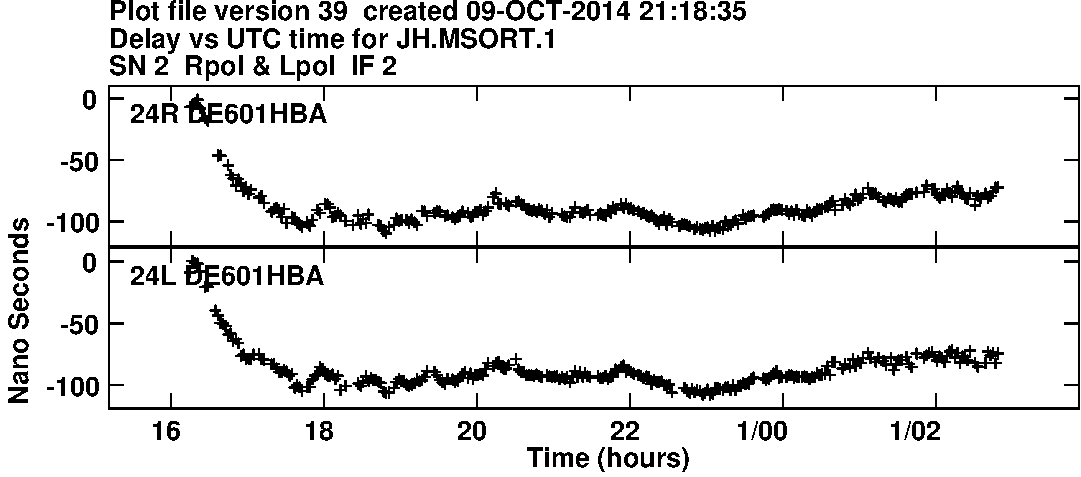
\includegraphics[width=0.75\textwidth]{figures/J0958Hdelays-crop.pdf}
%\label{fig:J0958Hdelays}
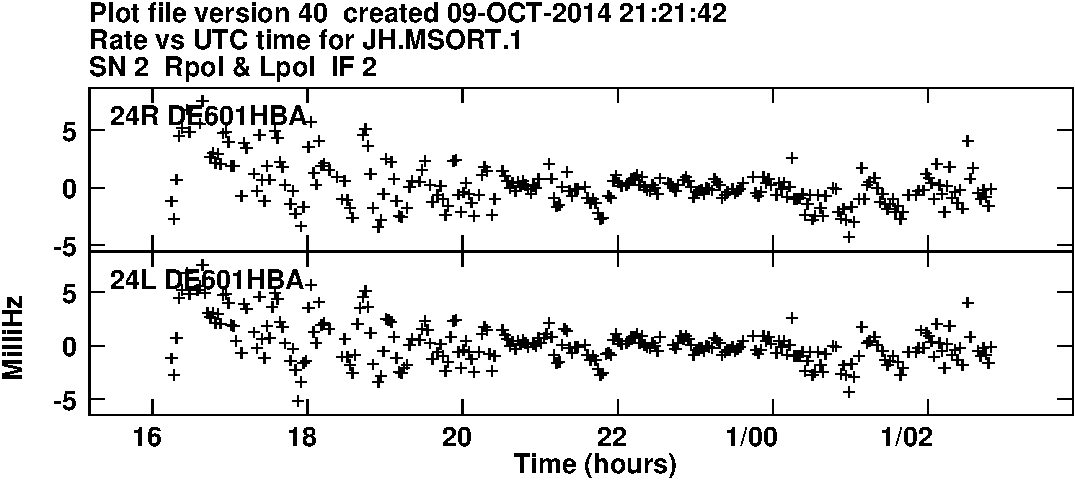
\includegraphics[width=0.75\textwidth]{figures/J0958Hrates-crop.pdf}
%\label{fig:J0958Hrates}
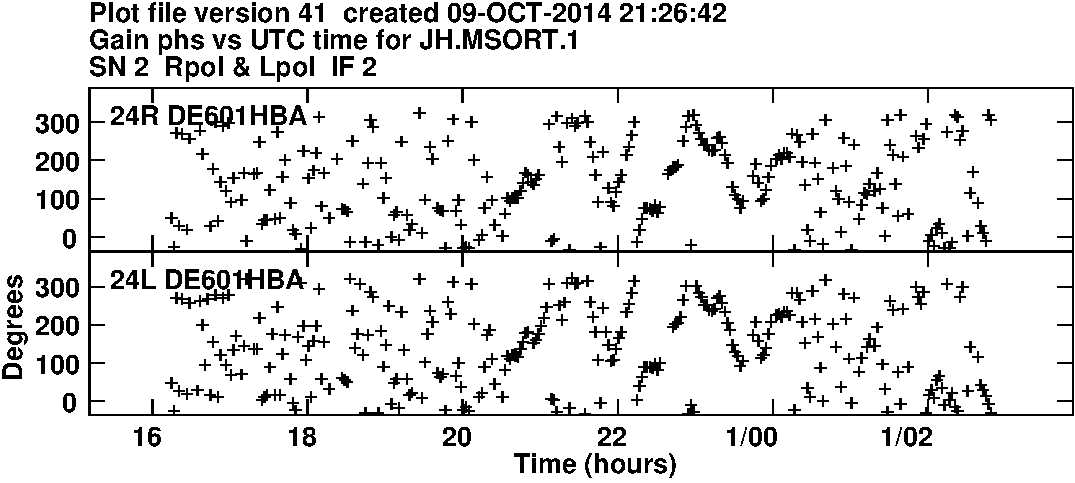
\includegraphics[width=0.75\textwidth]{figures/J0958Hfringpsol-crop.pdf}
%\label{fig:J0958Hfringphases}
\caption{
Delay (top), rate (middle) and phase(bottom) corrections derived for the source
J0958+6533 at 154\,MHz by FRING for antenna DE601HBA. These plots show the
corrections derived for a 10 hour observation (the first segment of project
LC0\_026). It is clear from the rates and phases that phases changes rapidly
during the first and last hours of the experiment. The delay solutions are more
stable, although there is a large change in at the start. In general, the
ionosphere is more stable during midnight than at sunset or sunrise.  }

\end{center}
\end{figure*}

% JM: For the final version we can think about a more compact plot with more stations, also to compare the behaviour of a RS and an IS.

\subsection{Amplitude calibration}

The amplitude calibration consists of finding the antenna gain factors
that scales the raw response of each antenna to the real flux density measured.
These scaling factors can be found calibrating the data with a bright source
with known flux density and structure (for example a point-like calibrator).
For core and remote stations, one can use, for example bright sources in low
frequency catalogs (such as MSSS). However, for International LOFAR that is in
general not possible because (1) there is not yet a catalogue of sources, and
therefore the structure of bright sources is unknown at this scales (2) the
international stations sample only very long $uv$ distances (see
Fig.~\ref{fig:uvcoverage}, right panel) that not overlap with the rest of the
array, which can be corrected, and (3) compact and bright regions of potential
calibrators, usually AGN, are expected to change with time. In principle,
instrumental gains within LOFAR could be tracked with time (this option is
currently being commissioning with the COBALT correlator), but since this
option is not yet available, making a sufficiently  accurate a priori
calibration is also not feasible. Therefore, the current approach requires to
self-calibrate a bright calibrator to find its small-scale structure, and
bootstrap its flux density between the short and long baselines, assuming that
the low-resolution flux density of the source is stable and known. 
% JM: here include references for the amplitude calibration of the short
% baselines from a previous chapter of the book.

For a science observation, it is recommended to include runs on very a bright
and known calibrator (for instance 3C196 or 3C84) and a compact source
(for instance a cm-VLBI calibrator or a bright pulsar) to set the amplitude
scale, and link the short/long-baselines flux density, respectively. We
note that a proper amplitude calibration requires also a good model of the
spectral index of the reference calibrator.  

\section{Practical considerations}
\label{sec:practical}

\subsection{Shift+average}\label{sec:shift}

Given the high resolution obtained with the International LOFAR observations,
imaging of the region restricted by the time and frequency average of the data
with the long-baseline resolution (see Table~\ref{tab:res}), would require
high  would require a very high computational cost. If one is interested in
multiple objects within the station beam, one needs to phase-shift (and
re-project) the $uv$-data to each object before averaging. After correlation,
the full-resolution visibility dataset can be shifted and averaged multiple
times, to the positions of all the target sources and possibly to one or more
nearby calibrators. Starting during cycle three, it will be possible to request shifting and averaging of data to multiple phase centers within a
beam as a part of a normal observation.

\subsection{Distributing bandwidth on different sources}\label{sec:bandwidth}

It is possible to distribute LOFAR bandwidth over a number of beams to
simultaneously observe different regions of the sky. In particular, it is
possible to divide the bandwidth on target(s) and calibrator, which provides a
continuous source calibration without the need of regularly nodding from target
to calibrator. Another possibility is to distribute the bandwidth among a large
number of sources to search for suitable calibrations. For example one can
generate 30 beams to observe simultaneously 30 sources with 3~MHz bandwith as a
fast way to search for suitable calibrators \citep[see i.e.][]{moldon14}

To optimize the observation it is possible to use fewer subbands on the
calibrator, and thereby get more subbands, i.e. lower continuum noise, on the
target beam. To use fringe finding, we need to sample accurately the residual
delay/rate slope (and possibly curvature at low frequencies) present in the
data. This can be done with sparse sampling in frequency, where the optimal
coverage is achieved by spreading the subbands as a powerlaw density with
denser placement of subbands at lower frequencies. The advantage of this
approach is that more bandwidth can be placed on the target.  The disadvantage
is that the calibration becomes a bit more demanding. One reason for this is
that the UVFITS format used by AIPS (for running fringe fitting) requires data
in all channels.  If we do not have contigouse subband coverage in frequency,
we need to insert fake data and flag that (e.g. using NDPPP, see [**Ref. to
imaging cookbook?]) before reading the data into AIPS. This will cause an
increase in data volume which will slow down processing. Also, spreading the
subbands sparsely is always a risk in case your calibrator is weaker than you
think. A detailed discussion can be found in \cite{marti-vidal10}. The authors
analyse how to distribute subbands specifically for LOFAR observations for
optimal fringe detection.
% JM: in the current distribution this is the first mention to AIPS procedures,
% which will be explained later. Check for consistency.

\subsection{Form a combined station}

The huge difference between the $uv$ distances provided by core-core baselines
and international baselines makes it very difficult to produce images were the
very compact and the very diffuse emission can be analysed. When studying the
compact structure of a source, the shortest baselines do not add too much
information, whereas they difficult the calibration, for example because they
are sensitive to a much bigger area of the sky, potentially including hundreds
of bright sources up to several degrees away. The core stations can be added to
form a coherent ``tied station'' (TS001) that keeps the core sensitivity and
the long baselines to the international stations. Since the core stations share
the same clock and are under similar atmospheric conditions, only slow changes
in their amplitudes and phases are expected, and thus they can be calibrated by
observing a bright primary calibrator once every $\sim1$~hr. TS001 is formed by
summing baseline visibilities with the NDPPP task ``StationAdder''.  After this
step, all original visibilities with core-core baselines can be discarded using
the NDPPP task ``Filter'' to significantly reduce the data volume.

One important benefit of having a tied station is that it works as a very
sensitive station. This tied-array station aids in the derivation of
calibration solutions to the international stations with FRING, and can be used
as a reference station. In Fig.~\ref{fig:CSvsTS} we show calibrated amplitudes
and phases for some baselines from some remote stations to a single core
station and to the tied station formed by coherently combining 23 core stations.
% JM: The plot is not very nice, and does not give too much information. Maybe
% include CS-International and TS-International baselines to see some amp/phase
% variations? Maybe include some numbers on the dispersions?

\begin{figure}
%\sidecaption[t]
\begin{center}
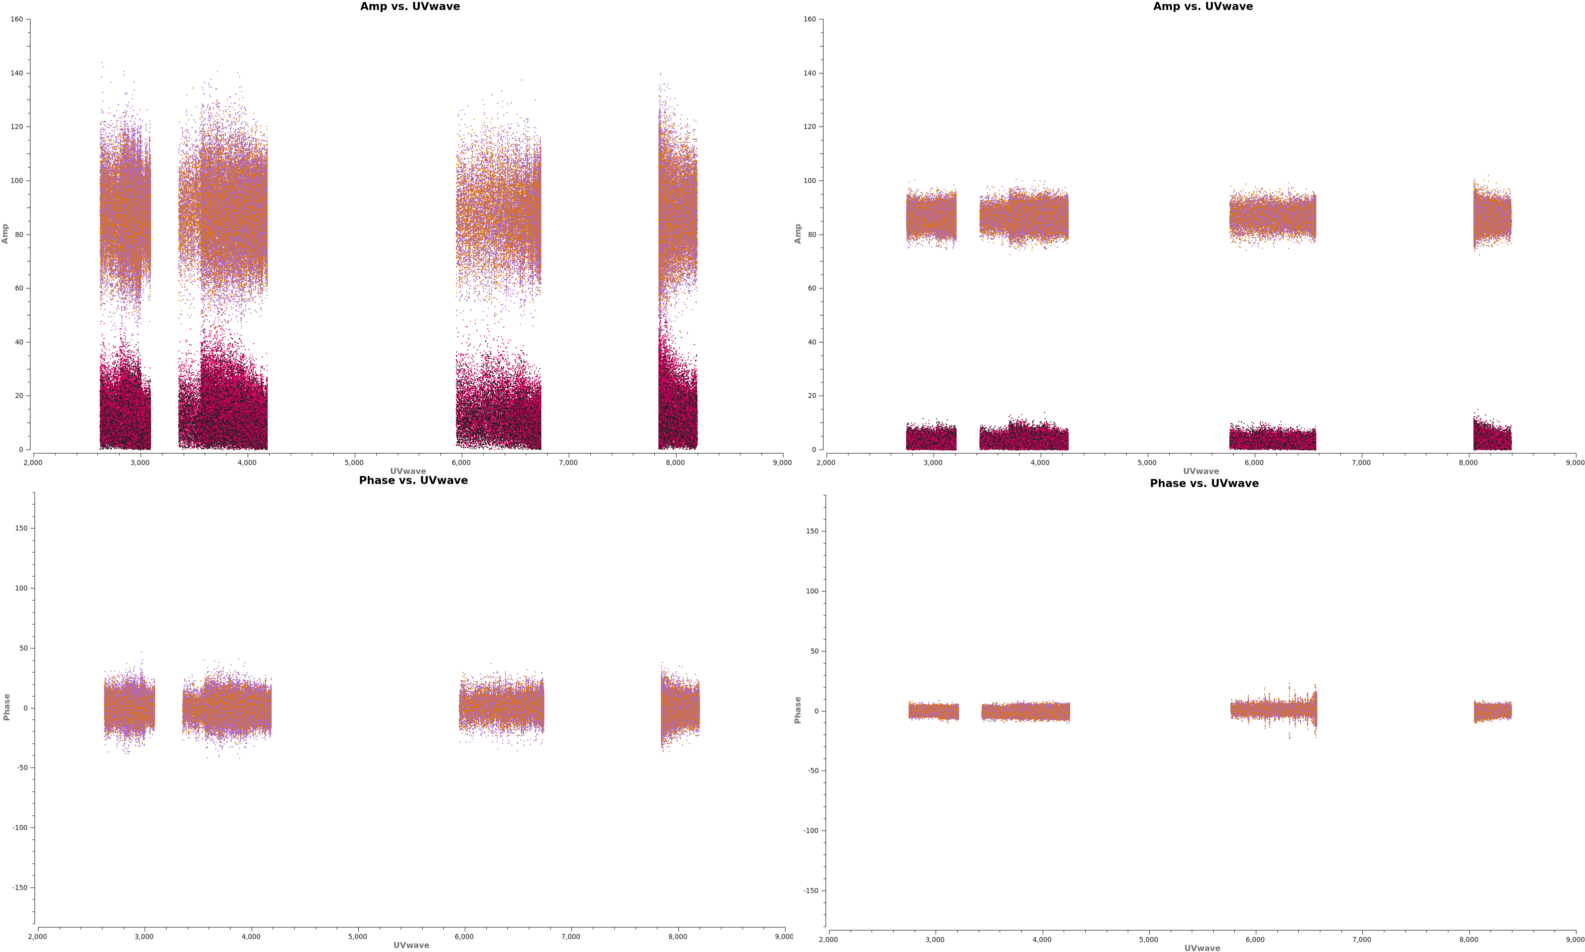
\includegraphics[width=\textwidth]{figures/amp_uv_CSRS_TSRS.png}
\caption{Amplitude (top) and phase (top) as a function of uv-distance for the
baselines between CS001 (left) and TS001 (right) to four remote stations.}
\label{fig:CSvsTS}
\end{center}
\end{figure}


\subsection{Linear to circular polarization}

Differential Faraday rotation introduces rapid phase changes with frequency
into linear polarisation data on long baselines. For long-baseline observations
is preferable to work in a circular (R,L) polarisation basis. In this basis,
the ionospheric disturbances are transformed from coupled amplitude/phase
effects (as in the linear X,Y basis) to phase only effects. Since differential Faraday rotation does not mix R and L
polarisations we may calibrate RR and LL independently. Furthermore, standard VLBI techniques like fringe fitting work in a circular (R,L)
polarisation basis. Therefore, the data have to be converted to circular polarisation before the phase calibration of the long baselines.
% JM: this paragraph can be more clear and straightforward.

Conversion to circular polarisation can be done using the Table Query Language
(TAQL) to operate on the measurement set data directly. We note that the
effects of the station beam should be calibrated with BBS before converting the
data. As the effects of the station beam were already calibrated, this is a
simple operation. However, we note that since BBS calibrates the XX and YY
components independently, an overall phase-offset between X and Y may remain. Another tool to convert from linear to circular polarisation is \emph{mscorpol} v1.6, developed by T. D. Carozzi.


% JM: it is recommended to use BBS corrections + taql conversion over mscorpol. The main reason is because eventually the beam model in BBS should be more accurate. Other reasons are that they are official LOFAR tools, that will probably get more maintenance, and have some additions, such as accounting for failing tiles, etc.  

%The M82 data \cite{varenius2014} were converted from linear to circular using
%the tool \emph{mscorpol} v1.6, developed by T. D. Carozzi.  This tool
%includes corrections for dipole-projection effects as a function of the
%correlated sky position relative to all included LOFAR stations.  After the
%conversion, the data are circularly polarised, with full (but approximated)
%parallactic angle correction. 

\subsection{Convert to UVFITS}

Since AIPS understands the UVFITS-format, but not Measurement Sets (MS)
we need to convert the data from MS to UVFITS. There are several ways to do this:
\begin{itemize}
\item You may use the function \emph{exportuvfits} in CASA.
\item You may use the tool \emph{ms2uvfits} available at the LOFAR cluster, as {\tt ms2uvfits in=[input-MS] out=[output-FITS-file] writesyscal=False}
\end{itemize}
Note that in a UVFITS file there MUST be data for all baselines included, although
data can be flagged if baselines are bad. If one tries to reduce data size by exluding particular subarrays
with NDPPP one may run into very strange errors in AIPS, since the basic assumptions of UVFITS are not valid.
Hence, it is important to ensure that data are contigous in frequency (e.g. by inserting fake data as explained above)
and that there are data present for all baselines in the dataset. 

The AIPS task FITLD can be used to load the data in to AIPS. For LOFAR data,
the parameters digicor=-1 and douvcomp=-1 should be used.


\subsection{Brief instroduction to calibration tables in AIPS}\label{sec:aips}

In AIPS one calibrates data by sucessively finding and improving corrections
for the amplitude and phase of visibilites. These corrections are stored in
tables.  Each correction derived is store in an 'SN' table, and the cumulative
corrections are stored in a 'CL' table. The SN table will have a resolution
which you specify for each task, i.e. if you find corrections averaging data in
two minute chunks, the SN table will have one value every two minutes. The CL
table may have a different granularity, so that when applying a specific SN
table, you may (automatically) interpolate to CL-table entries between the SN
entries. When you are done with calibration, the CL-table including all your
corrections can be multiplied with your data using the task SPLIT to produce a
UVFITS file with the corrected data.

\section{Finding calibrators}

Until a good catalogue of compact sources at MHz frequencies is available, it
is important to take into account that a science observation might require a
previous search of calibrators. A fast method using the distribution of
bandwidth between many sources (see Sect.~\ref{sec:bandwidth}) is described in
\cite{moldon14}. A pre-selection based on a number of parameters from existing
catalogues, such as the low-frequency spectral index, and the flux, ca be
performed to optimize the search. In particular the most useful catalogues are
the VLSS, at 74~MHz, 4~m wavelength \citep{lane12a}, the WENSS catalogue at
325~MHz, 92 cm wavelength \citep{rengelink97}, and, specially The
Multifrequency Snapshot Sky Survey (MSSS), which comes from LOFAR observations
\citep{heald14}. 

\cite{moldon14} showed that a density of $\sim1$ good calibrator per square
degree based on two fields with Galactic latitudes of $+26.6^{\circ}$ and
$+43.4^{\circ} $. However, we expect less compact sources at lower Galactic
latitudes due to interstellar scattering. The Galactic electron density model
NE2001 \citep{cordes02} predicts an scattering at a galactic latitude of
$50^{\circ}$ of almost 100~mas at 150~MHz, which is five times smaller than our
resolution. However, the scattering is about 300~mas, similar to our beamsize,
at latitudes of 5--10$^{\circ}$, depending on the longitude. Therefore,
observations below a Galactic latitude of 10$^{\circ}$ are likely to be
affected by scattering on the longest baselines, and the effect should be
severe below about 2$^{\circ}$, especially towards the Galactic Center. 




\section{Observing strategy}

For cm VLBI, the dispersive delay due to the ionosphere is small (and so are the
changes with time), meaning that solution intervals of duration minutes and
width tens to hundreds of MHz are generally permissible.  After application of
the solutions from the primary calibrator, it is common to use a secondary
calibrator\footnote{A secondary calibrator is often referred to as an
``in-beam'' calibrator if it is close enough to the target source to be observed
contemporaneously} closer to the target source (separation $\sim$arcmin), or to
use the target source if it is bright enough for ``self-calibration'', solving
only for the phase (no delay or rate). This second phase-only calibration is
used to refine the calibration errors that result from the spatial or temporal
interpolation of the primary solutions.  Because this is a problem with fewer
degrees of freedom, lower signal-to-noise ratio (S/N) data can be used.
Additionally, because the bulk delay has already been removed, even more
bandwidth can be combined in a single solution for a further improvement in S/N.
A secondary calibrator can therefore be considerably fainter (usually $\sim$1-10
mJy versus $>$100 mJy for a primary calibrator).  This typical VLBI calibration
strategy is illustrated in Figure~\ref{fig:calstrategy}.

\begin{figure*}[] %figure1
\center
%\resizebox{1.0\hsize}{!}{
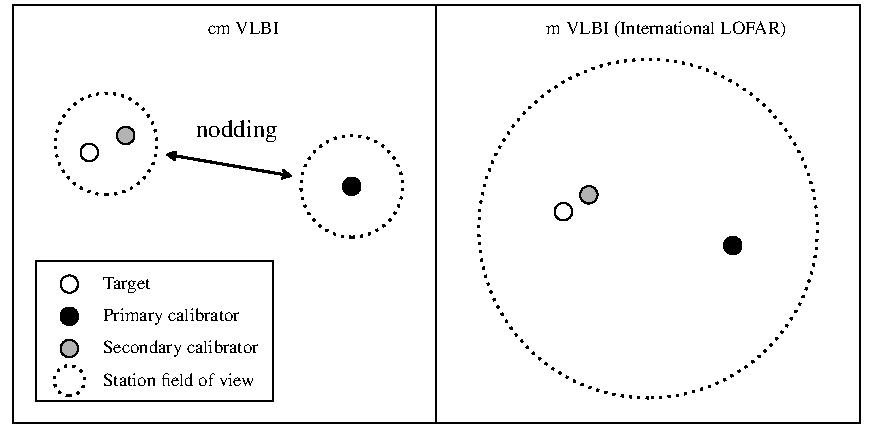
\includegraphics[width=\textwidth]{figures/vlbi_sketch.pdf}
%}
\caption{Typical calibration setup for cm VLBI (left) and International LOFAR
(right).  Note that in some cases the target may itself function as the
secondary calibrator.  A secondary calibrator is not always required for cm
VLBI, but will almost always be needed for International LOFAR, unless the
primary calibrator is fortuitously close.  The larger field of view of LOFAR
means that both the primary and secondary calibrators will always be observed
contemporaneously, unlike in cm VLBI, where nodding between the primary
calibrator and target is typically required (shown by the double arrow in the
left panel).}
\label{fig:calstrategy}
\end{figure*}


We propose the following approach for an International LOFAR observation: 
\begin{enumerate}
\item Identify candidate primary calibrators up to separations of a few degrees 
by using any of the criteria discussed in Sect.~\ref{results};
\item Conduct a short observation in snapshot mode as described
in Sect.~\ref{sec:obs} before the science observation to identify
the best primary calibrator (or calibrators).
\item If required and time permits, follow up with a ``full bandwidth'' snapshot observation to 
identify one or more secondary calibrators;
\item Set up the scientific observation to dwell on the field 
containing the primary calibrator and the target/secondary calibrator;
\item Include periodic scans (every $\sim$ hour) on a bright Dutch array 
calibrator to calibrate the core stations in order to form the tied station.
\item Shift phase centre to primary calibrator, preprocess and obtain delay solutions 
as described in this paper, apply them to the unshifted dataset;
\item If a secondary calibrator is to be used and is not yet identified, select 10 minutes
of data and perform shift/averaging to candidate secondary calibrator sources;
\item If secondary calibrator is used: shift and average primary-calibrated dataset, 
image and selfcalibrate, apply solutions to the unshifted dataset;
\item Shift and average calibrated dataset, image and (if needed) selfcalibrate target.
\end{enumerate}

In the near future, the pipeline used for this project will be developed, in
collaboration with the LOFAR operations team, into an expanded form capable of
carrying out the approach described above.  This pipeline will be made available
to all International LOFAR observers, delivering a reduced data volume for
long-baseline observations and enabling calibrated data to be more quickly
produced.


\begin{figure}
%\sidecaption[t]
\begin{center}
\includegraphics[width=\textwidth]{figures/{4C19.44_165MHz_lowres+highres}.png}
\caption{Example of nice image produced with the long baselines. We have to find something.}
\label{fig:fog}
\end{center}
\end{figure}







\begin{acknowledgement}
Thanks to people. Other thanks.

AIPS is produced and maintained by the National Radio Astronomy
Observatory, a facility of the National Science Foundation
operated under cooperative agreement by Associated Universities, Inc.

\end{acknowledgement}

%\input{references01}

\bibliographystyle{aa}
\bibliography{chapter13}

\end{document}
